\appendix
\chapter{Solved Examples}

Some useful solved examples from the book ``Microelectronics Circuits - Theory and Applications", Fifth Edition by Adel S.Sedra and Kenneth C. Smith, Adapted by Arun N Chandorkar (Oxford University Press) are presented in the Appendix.

\section {Diode}
\begin{enumerate}
\item \textbf {Example 2.1:} Figure \ref{sch1} shows a circuit for charging a 12-V battery. If $v_s$ is a sinusoid with 24-V peak amplitude, find the fraction of each cycle during which diode conducts. Also, find the peak value of the diode current and the maximum reverse-bias voltage that appears across diode.

\textbf {Solution:} Draw the schematic shown in Figure \ref{sch1} using schematic editor.
\begin{figure}%h stands for 'here'. If h is removed then the fig will go to the bottom or to the next page.
\begin{center}
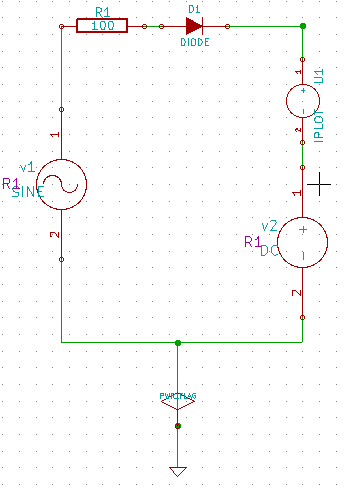
\includegraphics[width=0.5\linewidth]{figures/apd1.png}%If the fig is appearing too big/small, change the scaling factor 0.2
\caption{Schematic of example 2.1}
\label{sch1}
\end{center}
\end{figure}
Annotate the schematic using the \textit{Annotate} tool from the top toolbar in Schematic editor. Perform Electric Rules check using the \textit{Perfrorm electric rules check} tool from the top toolbar. Ensure that there are no errors in the circuit schematic. Now generate Spice netlist for simulation using the \textit{Generate Netlist} tool from the top toolbar. This is shown in Figure \ref{apd4}.

\begin{figure}
\begin{center}
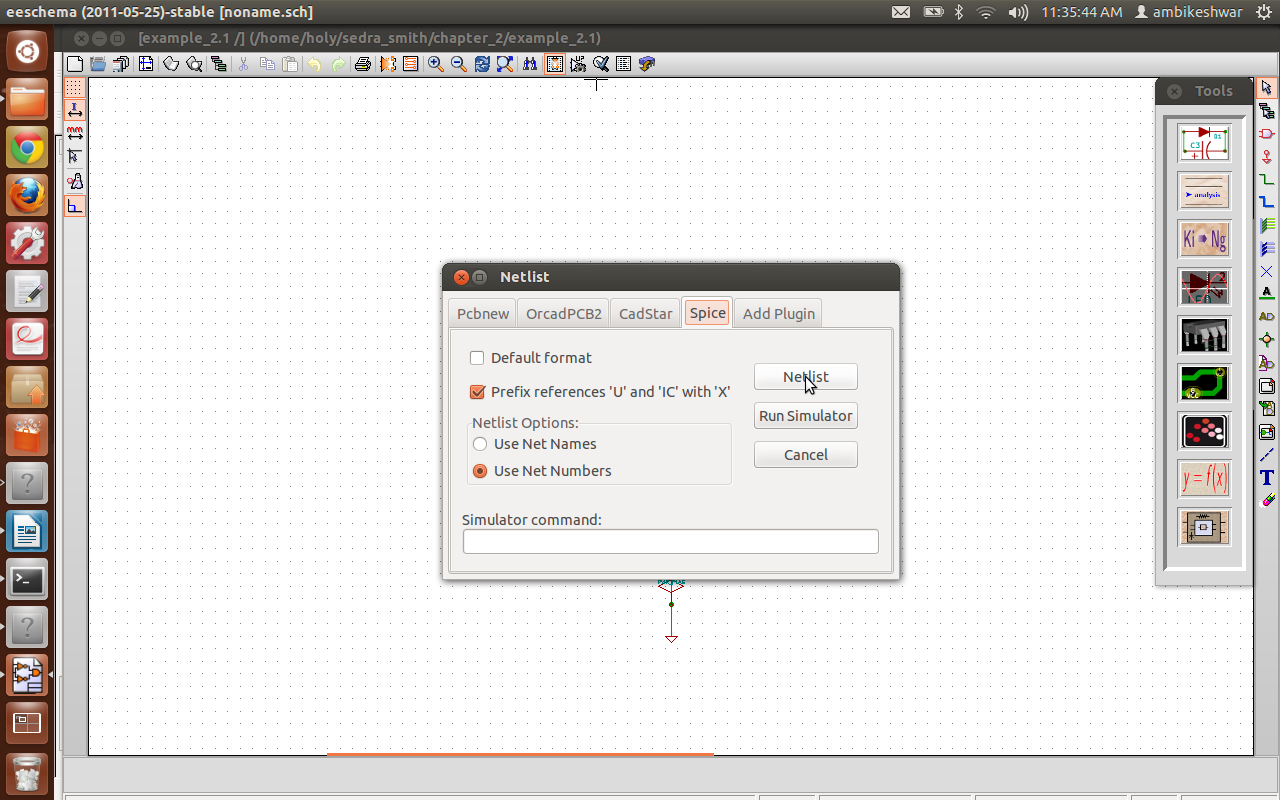
\includegraphics[width=0.7\linewidth]{figures/apd4.png}
\caption{Netlist generation}
\label{apd4}
\end{center}
\end{figure}


The next step is to invoke 
Analysis inserter from the Oscad tool bar. Click {\tt analysis inserter} and select the option {\tt transient} as given in Figure \ref{apd6}.
\begin{figure}
\begin{center}
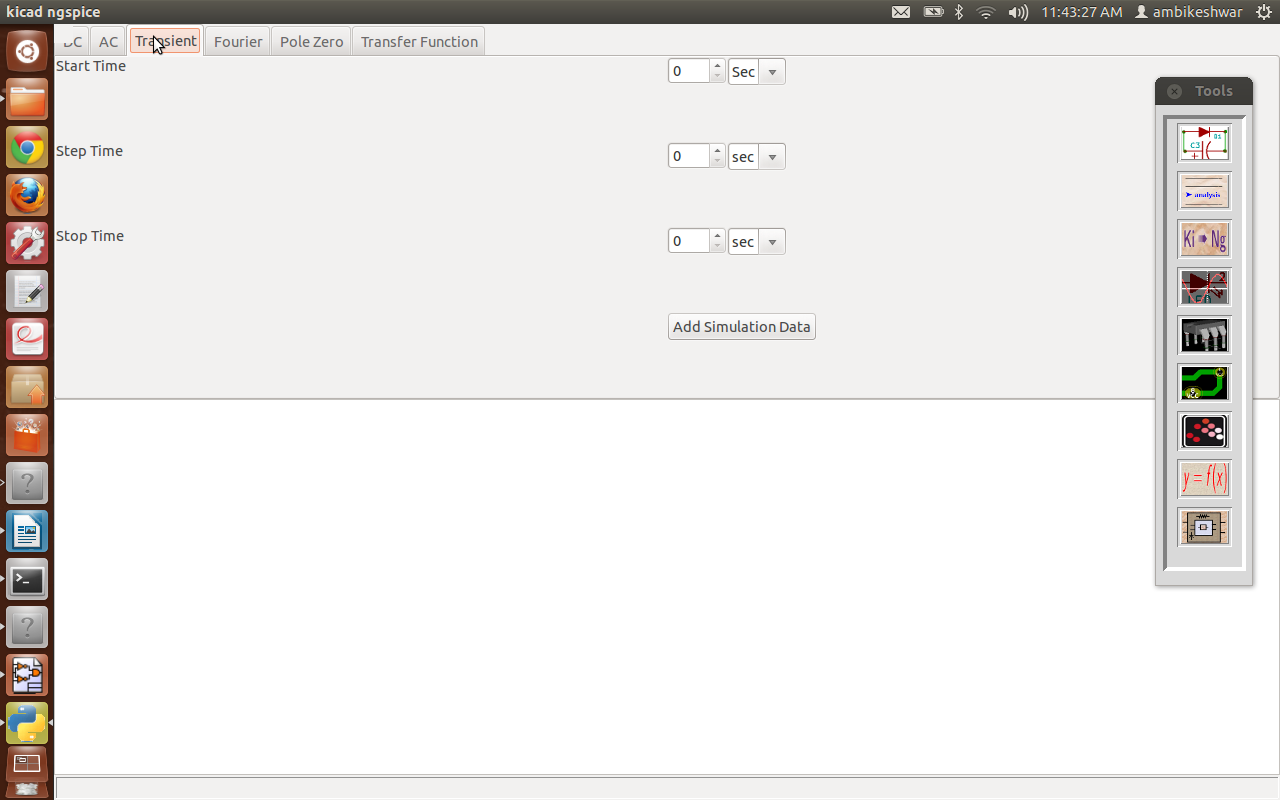
\includegraphics[width=0.5\linewidth]{figures/apd6.png}
\caption{Analysis Inserter}
\label{apd6}
\end{center}
\end{figure}
Enter {\tt start time} = 0, {\tt step time} = 1 ms, {\tt stop time} = 10 ms as in Figure \ref{apd7}.

\begin{figure}%h stands for 'here'. If h is removed then the fig will go to the bottom or to the next page.
\begin{center}
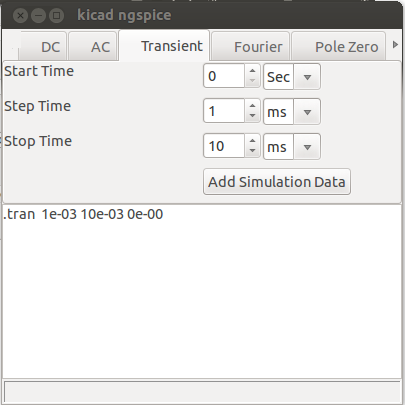
\includegraphics[width=0.7\linewidth]{figures/apd7.png}%If the fig is appearing too big/small, change the scaling factor 0.2
\caption{Analysis Inserter: Transient simulation options}
\label{apd7}
\end{center}
\end{figure}
Click on {\tt Add Simulation Data} and save the analysis file as in figure \ref{apd8}.

\begin{figure}%h stands for 'here'. If h is removed then the fig will go to the bottom or to the next page.
\begin{center}
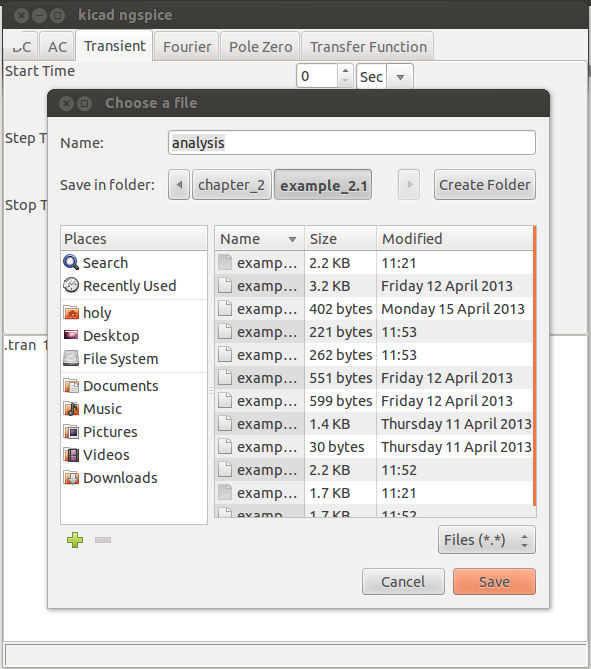
\includegraphics[width=0.7\linewidth]{figures/apd8.png}%If the fig is appearing too big/small, change the scaling factor 0.2
\caption{Analysis Inserter: Save analysis file}
\label{apd8}
\end{center}
\end{figure}

Now click on {\tt Netlist Converter} in Oscad tool bar and enter the values of DC source and {\tt SINE} source as shown in following figure \ref{apd9}
\begin{figure}
\begin{center}
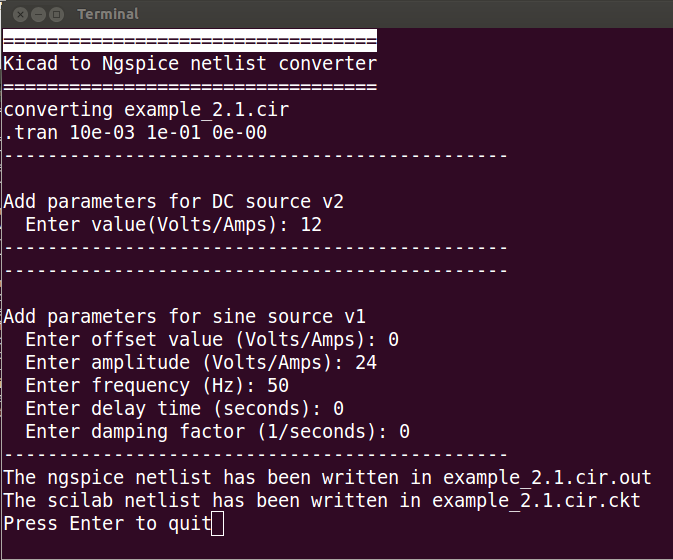
\includegraphics[width=1\linewidth]{figures/apd9.png}
\caption{Kicad to Ngspice}
\label{apd9}
\end{center}
\end{figure}
and then press `enter' key. This will generate the Ngspice netlist (.cir.out).

Now click on {\tt Ngspice} from the Oscad tools bar. This will open up the Ngspice terminal with waveform window as shown in figure \ref{apd10}.

\begin{figure}
\begin{center}
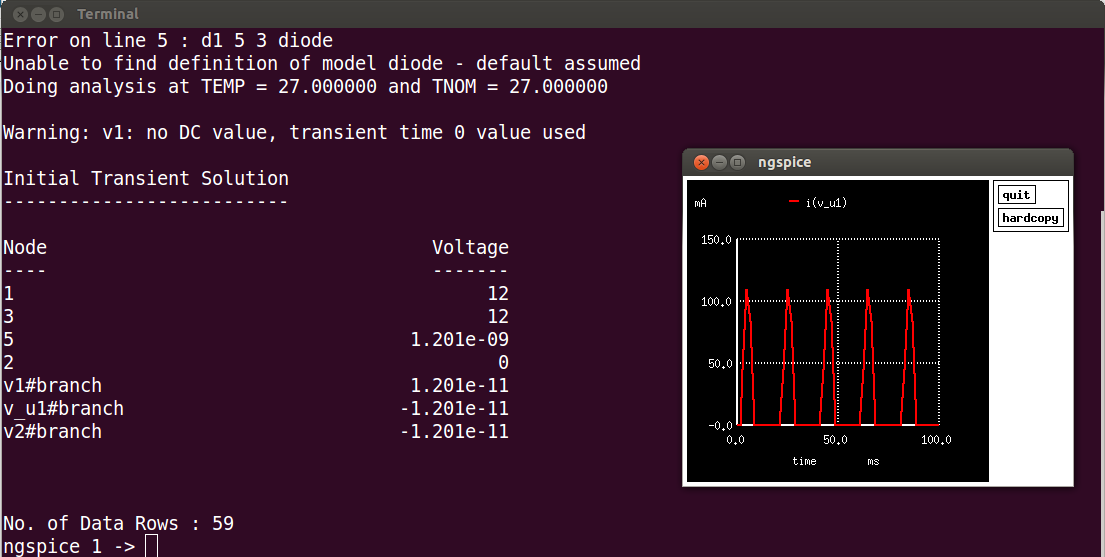
\includegraphics[width=1\linewidth]{figures/apd10.png}
\caption{Ngspice Waveform Window}
\label{apd10}
\end{center}
\end{figure}

\item \textbf {Example 2.5:} Find the voltage $V_D$ and current $I_D$ in the circuit shown in Figure \ref{apd11}, where $V_{DO}$ = 0.65, $r_D$ = 20 $\Omega$.\\

\textbf {Solution:} Create schematic and generate netlist in the same way as given in Example 2.1. 
\begin{figure}%h stands for 'here'. If h is removed then the fig will go to the bottom or to the next page.
\begin{center}
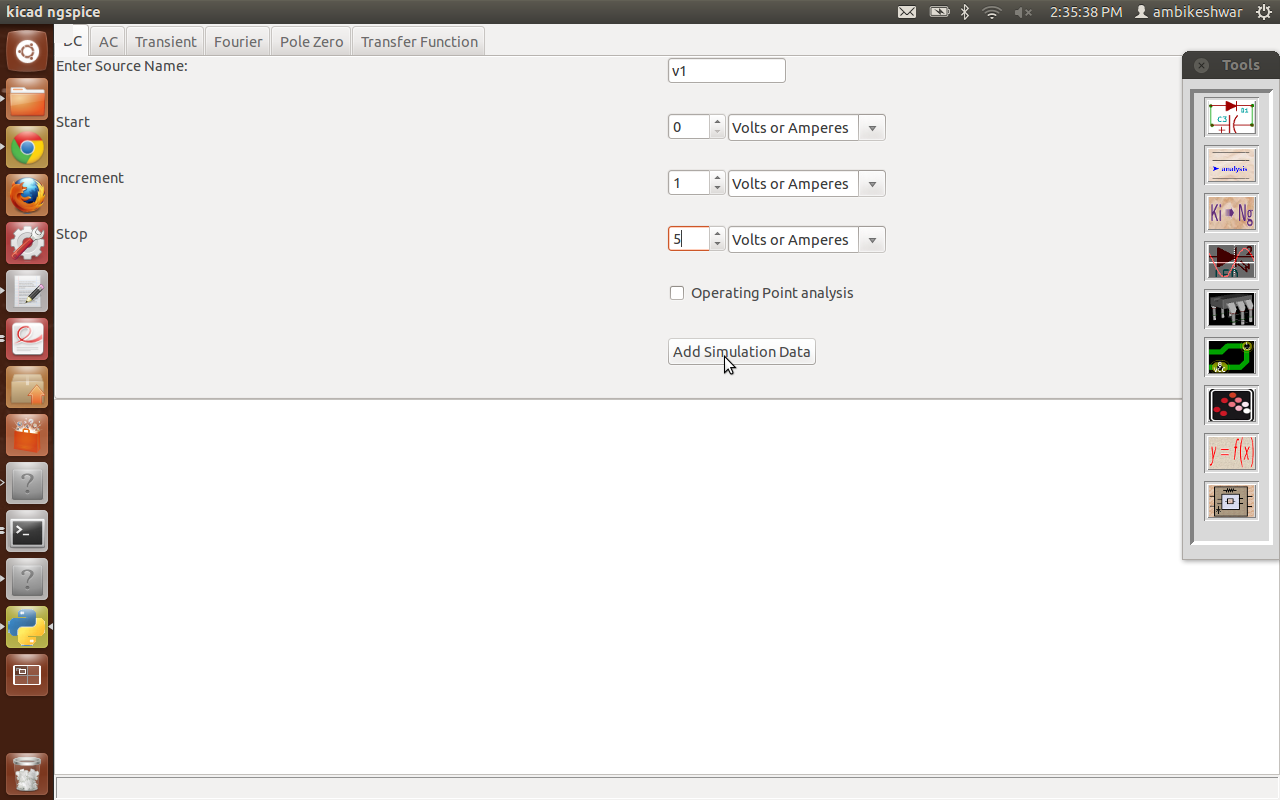
\includegraphics[angle=90, width=1\linewidth]{figures/apd11.png}%If the fig is appearing too big/small, change the scaling factor 0.2
\caption{Schematic}
\label{apd11}
\end{center}
\end{figure}

Click on ``analysis inserter" from Oscad tool bar. Select ``DC" and then enter the following details: {\tt enter source name} = v1, {\tt start} = 0, {\tt increment} = 1V and {\tt stop} = 5V as given in Figure \ref{apd12}. Click on ``Add Simulation Data" and save the analysis file.

\begin{figure}
\begin{center}
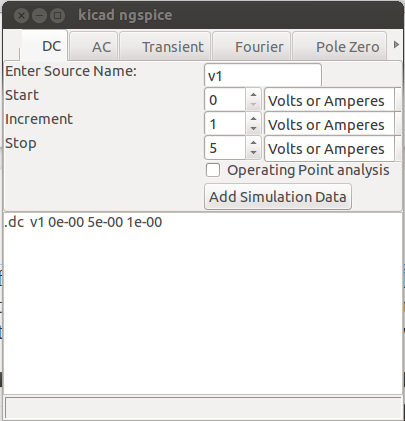
\includegraphics[width=0.7\linewidth]{figures/apd12.png}
\caption{Analysis Inserter}
\label{apd12}
\end{center}
\end{figure}

Now click on {\tt Netlist Converter} and enter the value of DC source as shown in Figure \ref{apd13} 
\begin{figure}
\begin{center}
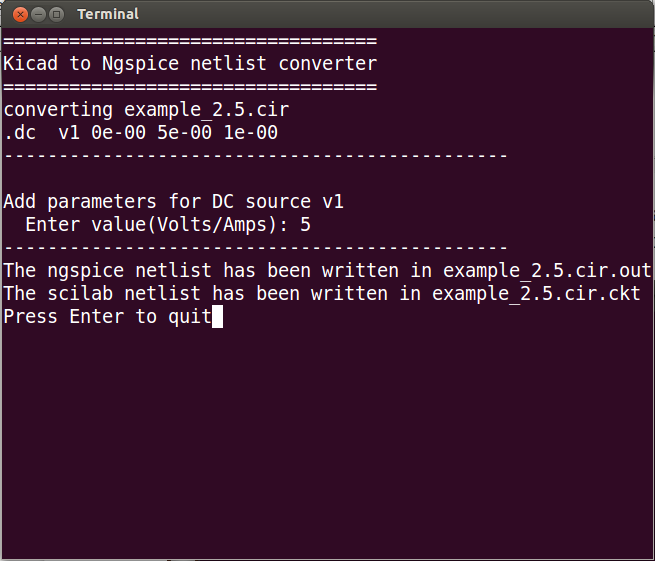
\includegraphics[width=1\linewidth]{figures/apd13.png}
\caption{Kicad to Ngspice}
\label{apd13}
\end{center}
\end{figure}
and then press `enter' key. Now click on ``Ngspice" from the Oscad tool bar. The results of Ngspice simulation is shown in Figure \ref{apd14}.
\begin{figure}
\begin{center}
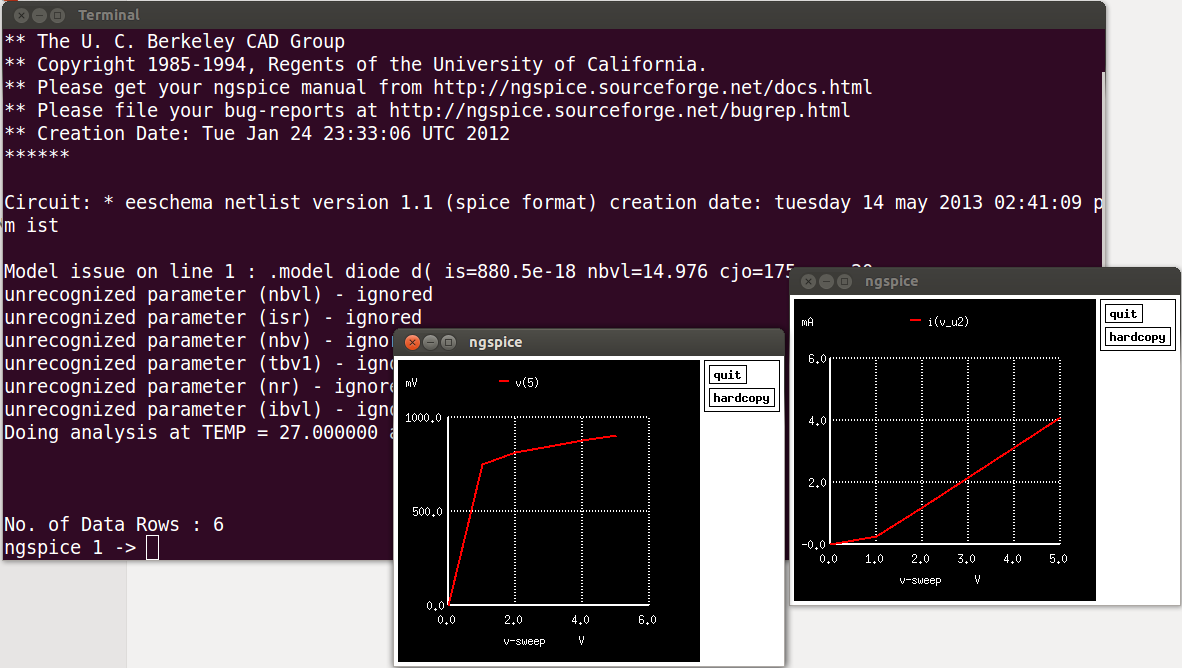
\includegraphics[width=1\linewidth]{figures/apd14.png}
\caption{Ngspice Waveform window}
\label{apd14}
\end{center}
\end{figure}
This shows the current and voltage waveforms and Ngspice terminal.
\end{enumerate}
\section {BJT}

\textbf{Example 3.1:} Find the voltage at all nodes in the transistors shown in Figure \ref{apd15}. We will assume that $\beta$ is specified to be 100.\\


\textbf{Solution:}  Create schematic and generate netlist in the same way as given in Example 2.1. 
         

\begin{figure}%h stands for 'here'. If h is removed then the fig will go to the bottom or to the next page.
\begin{center}
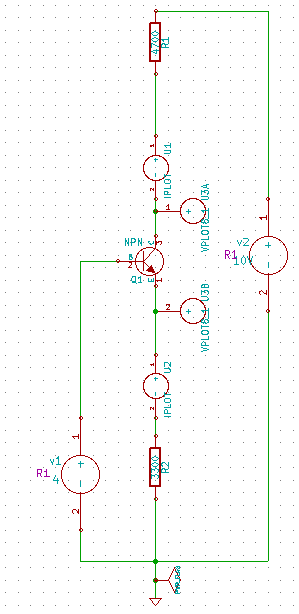
\includegraphics[angle=90,width=\linewidth]{figures/apd15.png}%If the fig is appearing too big/small, change the scaling factor 0.2
\caption{Schematic}
\label{apd15}
\end{center}
\end{figure}

Click on ``analysis inserter" from Oscad tool bar.
select ``DC" and then enter the following details:
{\tt enter source name} = v1, {\tt start} = 0, {\tt increment} = 1V and {\tt stop} = 15V as given in Figure \ref{apd16}. Click on ``Add Simulation Data" and save the analysis file. 
\begin{figure}
\begin{center}
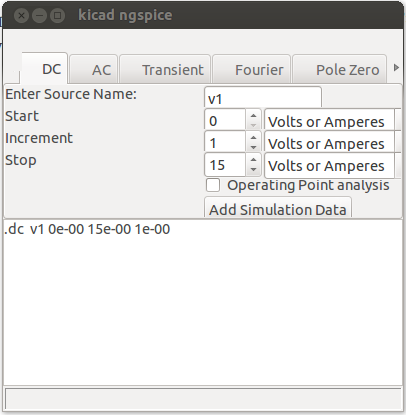
\includegraphics[width=0.5\linewidth]{figures/apd16.png}
\caption{Analysis Inserter}
\label{apd16}
\end{center}
\end{figure}
Now click on {\tt Netlist Converter} and enter the value of DC source as shown in Figure \ref{apd17}
\begin{figure}
\begin{center}
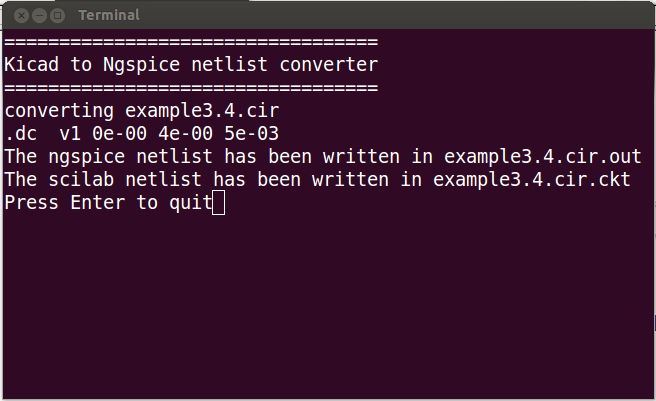
\includegraphics[width=0.6\linewidth]{figures/apd17.png}
\caption{Kicad to Ngspice}
\label{apd17}
\end{center}
\end{figure}
and then press `enter' key. Now click on ``Ngspice" from the Oscad tool bar. The results of Ngspice simulation is shown in Figure \ref{apd18}.
\begin{figure}
\begin{center}
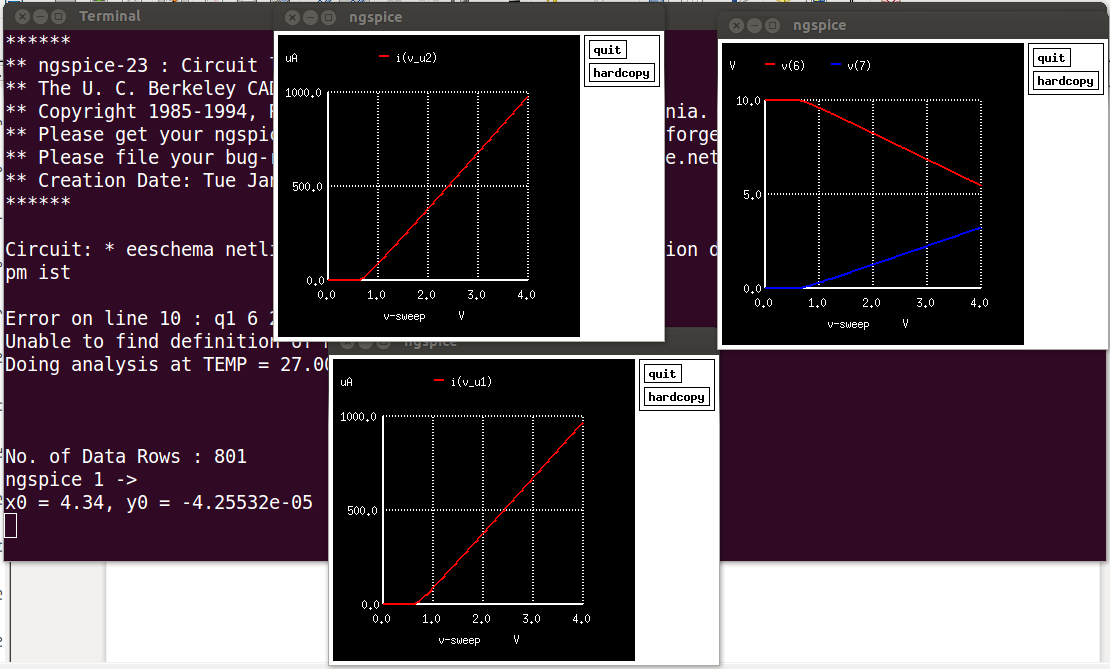
\includegraphics[width=1\linewidth]{figures/apd18.png}
\caption{Ngspice Waveform}
\label{apd18}
\end{center}
\end{figure}
\section {MOSFET}
\textbf{Example 4.5:} Analyze the circuit shown in fig \ref{mos1} to determine the voltages at all nodes and the current through all branches. \\


\textbf{Solution:} Create schematic and generate netlist in the same way as given in Example 2.1. 
        
\begin{figure}
\begin{center}
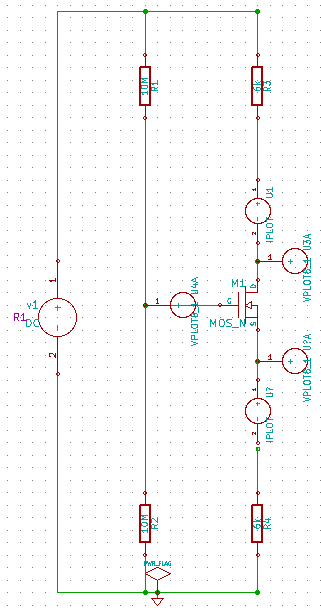
\includegraphics[angle=90,width=1\linewidth]{figures/mosfet1.png}%If the fig is appearing too big/small, change the scaling factor 0.2
\caption{Schematic}
\label{mos1}
\end{center}
\end{figure}

Click on ``analysis inserter" from Oscad tool bar.
select ``DC" and then enter the following details:
{\tt enter source name} = v1, {\tt start} = 0, {\tt increment} = 1V and {\tt stop} = 10V as given in Figure \ref{mos2}. Click on ``Add Simulation Data" and save the analysis file. 
\begin{figure}.
\begin{center}
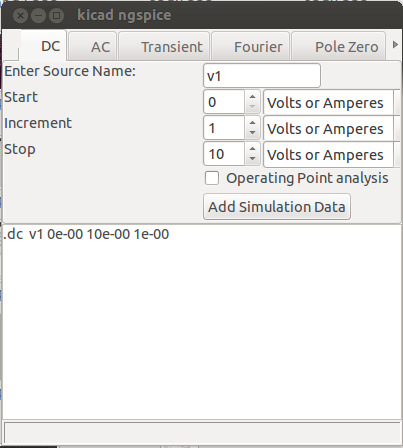
\includegraphics[width=0.6\linewidth]{figures/mosfet2.png}
\caption{Analysis Inserter}
\label{mos2}
\end{center}
\end{figure}
Click on ``Add Simulation Data" and save the analysis file.

Now click on {\tt Netlist Converter} and enter the value of DC source as shown in Figure \ref{mos3}.
\begin{figure}
\begin{center}
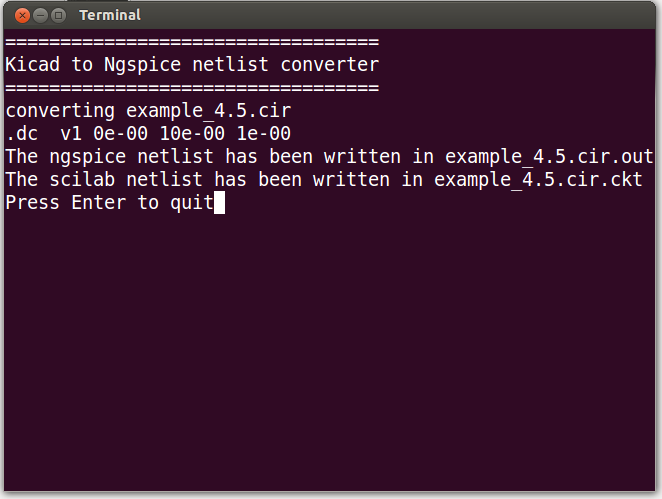
\includegraphics[width=1\linewidth]{figures/mosfet3.png}
\caption{Kicad to Ngspice}
\label{mos3}
\end{center}
\end{figure}
and then press `enter' key. Now click on ``Ngspice" from the Oscad tool bar. The results of Ngspice simulation is shown in Figure \ref{mos4}.

\begin{figure}
\begin{center}
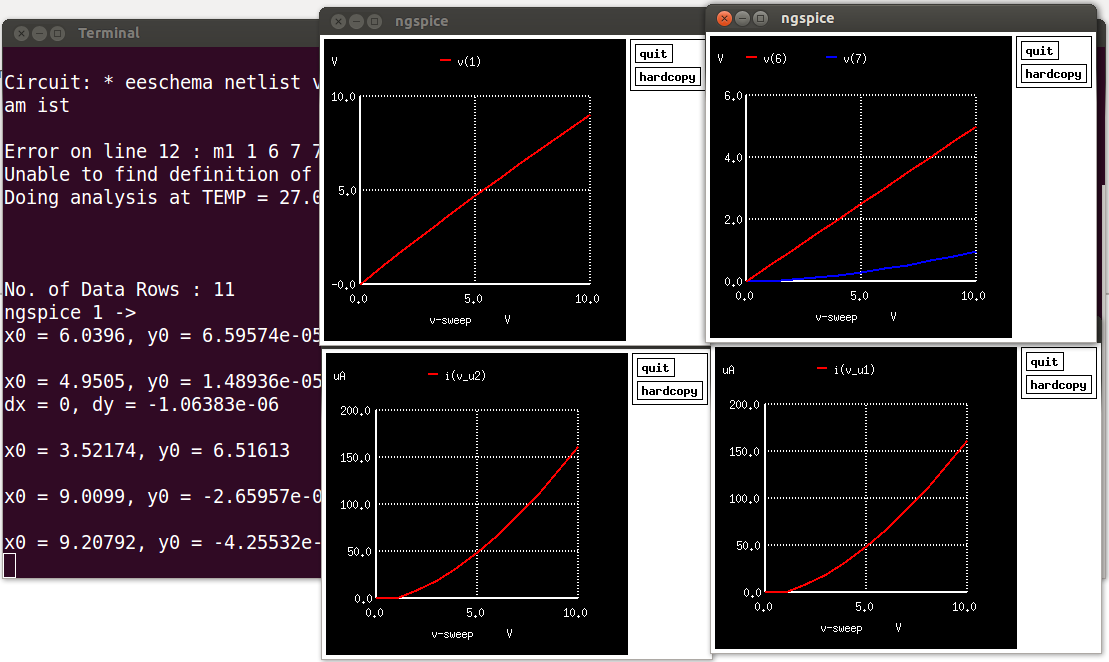
\includegraphics[width=1\linewidth]{figures/mosfet4.png}
\caption{Ngspice Waveform}
\label{mos4}
\end{center}
\end{figure}

\section {OP-AMP}
\begin{enumerate}
\item \textbf{Example 5.3:} Figure \ref{apd19} shows an op-amp circuit. Find the output voltage where $R_1$ = 10 $\Omega$, $R_f$ = 1k$\Omega$, $R_L$ = 100k$\Omega$ and input voltage $v_I$ = 10V.\\


\textbf{Solution:} Create schematic and generate netlist in the same way as given in Example 2.1. While generating netlist, DO NOT uncheck the option {\tt Prefix references `U' and `IC' with `X'}.

\begin{figure}%h stands for 'here'. If h is removed then the fig will go to the bottom or to the next page.
\begin{center}
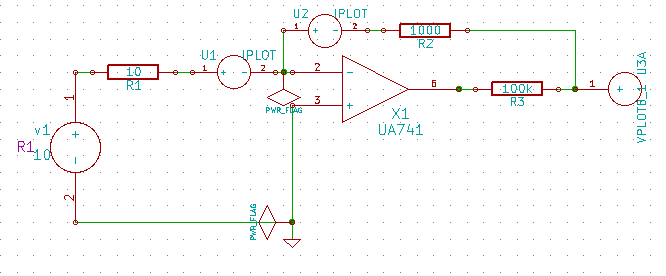
\includegraphics[width=0.7\linewidth]{figures/apd19.png}%If the fig is appearing too big/small, change the scaling factor 0.2
\caption{Schematic}
\label{apd19}
\end{center}
\end{figure}
Click on ``analysis inserter" from Oscad tool bar.
select ``DC" and then enter the following details:
{\tt enter source name} = v1, {\tt start} = 0, {\tt increment} = 1V and {\tt stop} = 10V as given in Figure \ref{mos2}. Click on ``Add Simulation Data" and save the analysis file. 


%\begin{figure}%h stands for 'here'. If h is removed then the fig will go to the bottom or to the next page.
%\begin{center}
%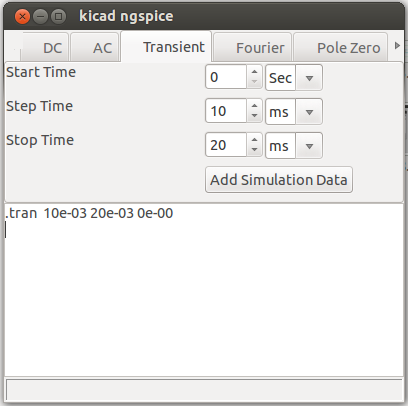
\includegraphics[width=1\linewidth]{figures/apd20.png}%If the fig is appearing too big/small, change the scaling factor 0.2
%\caption{Analysis Inserter}
%\label{20}
%\end{center}
%\end{figure}
Click on ``Subcircuit builder" from the Oscad toolbar and click on \textit{Cancel} in the subcircuit selector window. Now, \textit{import} the existing subcircuits. Figure \ref{21} will appear. Choose {\tt ua741} and click on \textit{ok}.
\begin{figure}%h stands for 'here'. If h is removed then the fig will go to the bottom or to the next page.
\begin{center}
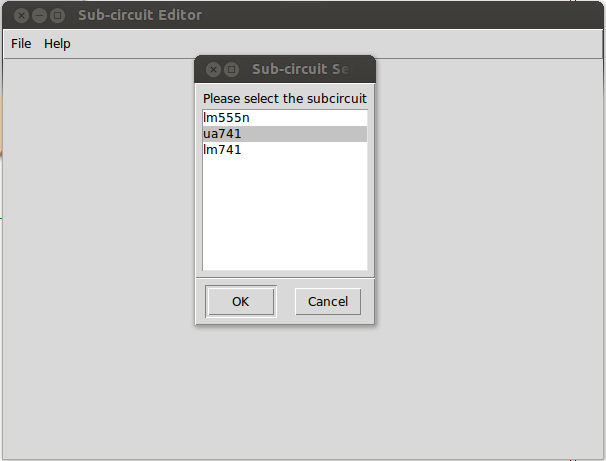
\includegraphics[width=1\linewidth]{figures/apd21.png}%If the fig is appearing too big/small, change the scaling factor 0.2
\caption{subcircuit builder 1}
\label{21}
\end{center}
\end{figure}
Figure \ref{22} will now appear.

\begin{figure}%h stands for 'here'. If h is removed then the fig will go to the bottom or to the next page.
\begin{center}
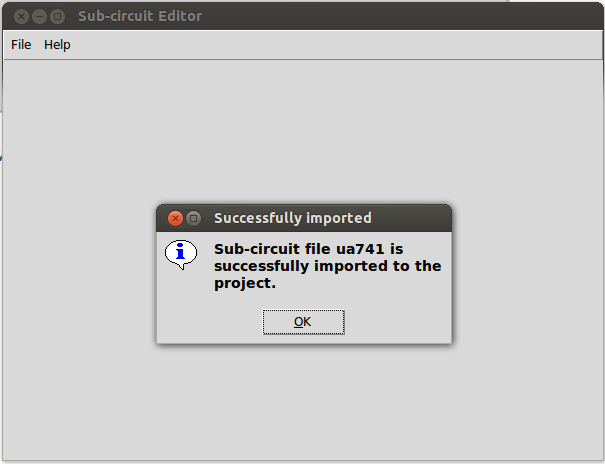
\includegraphics[width=1\linewidth]{figures/apd22.png}%If the fig is appearing too big/small, change the scaling factor 0.2
\caption{subcircuit builder 2}
\label{22}
\end{center}
\end{figure}

Click on ok in the {\tt Successfully imported} window. Let us open the subcircuit schematic of {\tt ua741}. This can be done as follows: Click on the \textit{File} menu. Choose \textit{open} and then type {\tt ua741} in the \textit{Enter Component name} field as shown in Figure \ref{openua741}. Click on ok.
\begin{figure}
\begin{center}
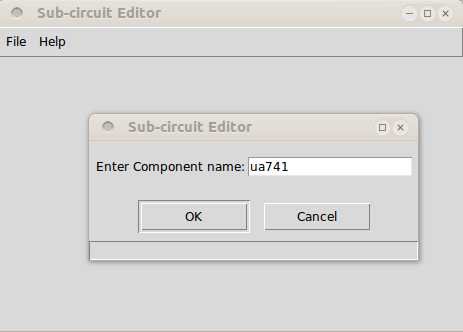
\includegraphics[width=1\linewidth]{figures/openua741.png}%If the fig is appearing too big/small, change the scaling factor 0.2
\caption{Open component subcircuit}
\label{openua741}
\end{center}
\end{figure}
Add the Oscad libraries to the subcircuit schematic to prevent the Load Error. The schematic of the subcircuit is as shown in Figure \ref{23}. 
\begin{figure}%h stands for 'here'. If h is removed then the fig will go to the bottom or to the next page.
\begin{center}
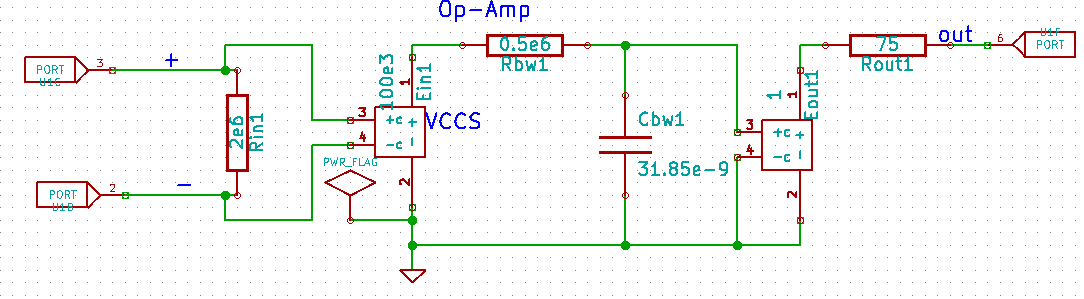
\includegraphics[width=1\linewidth]{figures/apd23.png}%If the fig is appearing too big/small, change the scaling factor 0.2
\caption{subcircuit builder 3}
\label{23}
\end{center}
\end{figure}

Now click on {\tt Netlist Converter} and enter the value of DC source as shown in Figure \ref{24} and then press 'enter' key. Now click on Ngspice button in Toolbar. The figure \ref{25} will appear.
\begin{figure}
\begin{center}
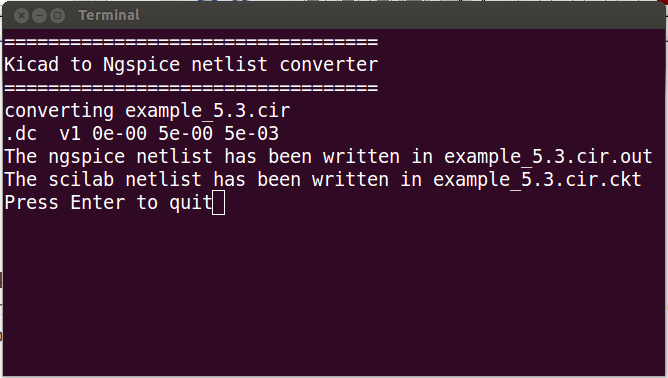
\includegraphics[width=1\linewidth]{figures/apd24.png}
\caption{Kicad to Ngspice}
\label{24}
\end{center}
\end{figure}

\begin{figure}
\begin{center}
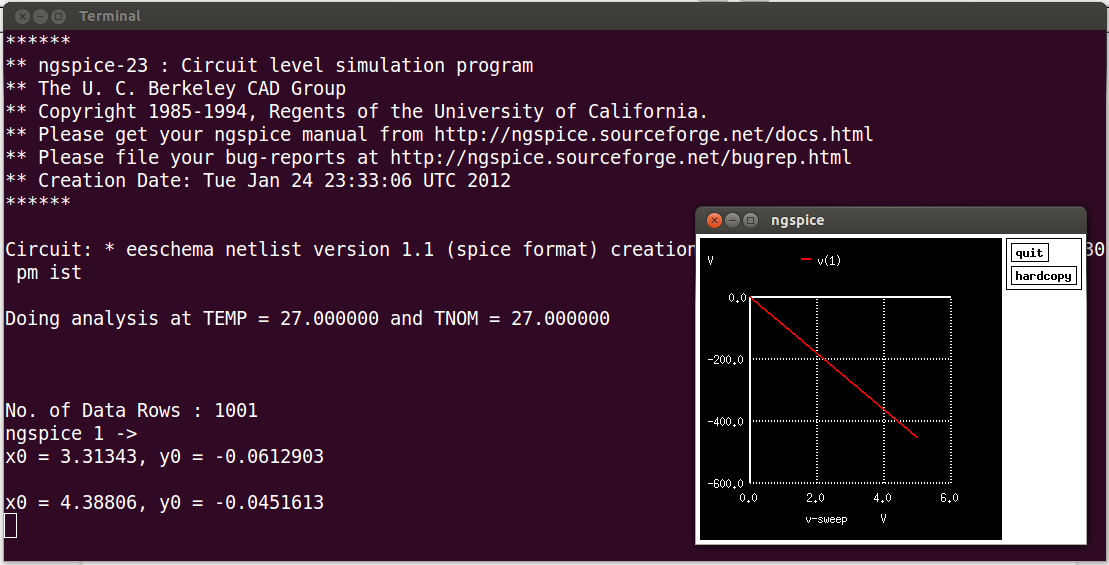
\includegraphics[width=1\linewidth]{figures/apd25.png}
\caption{Ngspice Waveform}
\label{25}
\end{center}
\end{figure}

\item \textbf{Example 5.6:} Consider the non inverting amplifier circuit shown in Figure \ref{26}. It is fed with a lower frequency sinusoidal signal of peak voltage $V_i$ = 1V, and is connected to load resistance $R_L$ = 1k$\Omega$.\\


\textbf{Solution:} Create schematic and generate netlist in the same way as given in Example 2.1.
\begin{figure}
\begin{center}
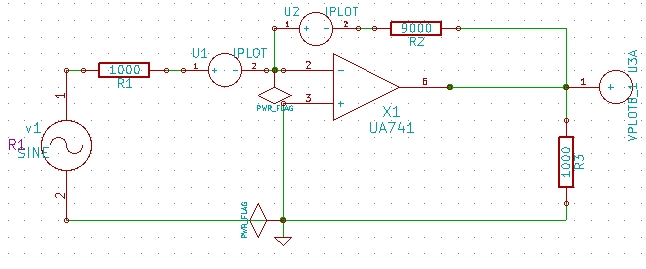
\includegraphics[width=1\linewidth]{figures/apd26.png}
\caption{Schematic}
\label{26}
\end{center}
\end{figure}

Click on ``analysis inserter" from Oscad tool bar.
select ``Transient" and then enter the following details:
{\tt Start time} = 0 sec, {\tt Step time} = 1 ms, {\tt stop time} = 10 ms as given in Figure \ref{27}. Click on ``Add Simulation Data" and save the analysis file. For subcircuit builder, follow the steps given in Example 5.3.
\begin{figure}%h stands for 'here'. If h is removed then the fig will go to the bottom or to the next page.
\begin{center}
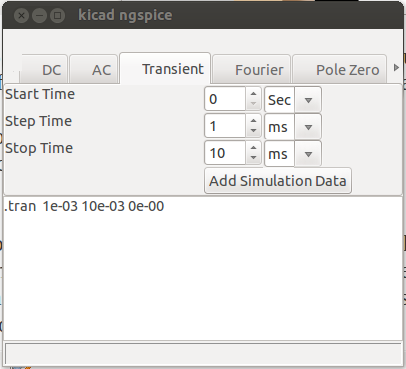
\includegraphics[width=1\linewidth]{figures/apd27.png}%If the fig is appearing too big/small, change the scaling factor 0.2
\caption{Analysis Inserter}
\label{27}
\end{center}
\end{figure}

Now click on {\tt Netlist Converter} and enter the value of sine source as shown in Figure \ref{31} and then press 'enter' key. Now click on Ngspice button in Toolbar. The figure \ref{32} will appear.
\begin{figure}%h stands for 'here'. If h is removed then the fig will go to the bottom or to the next page.
\begin{center}
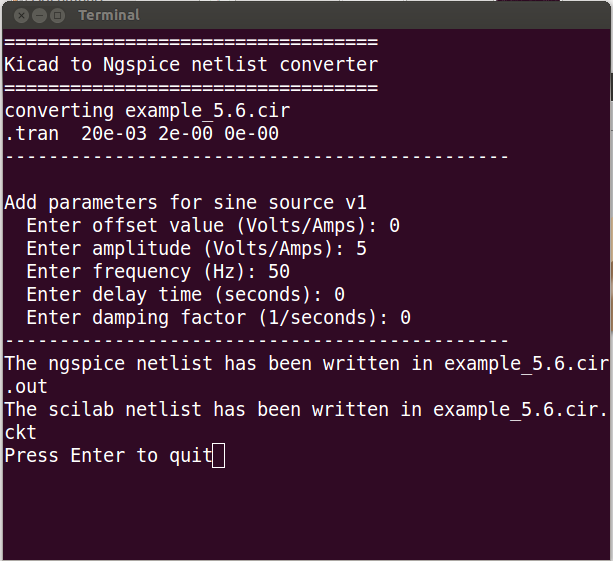
\includegraphics[width=1\linewidth]{figures/apd31.png}%If the fig is appearing too big/small, change the scaling factor 0.2
\caption{Kicad to Ngspice}
\label{31}
\end{center}
\end{figure}
\begin{figure}%h stands for 'here'. If h is removed then the fig will go to the bottom or to the next page.
\begin{center}
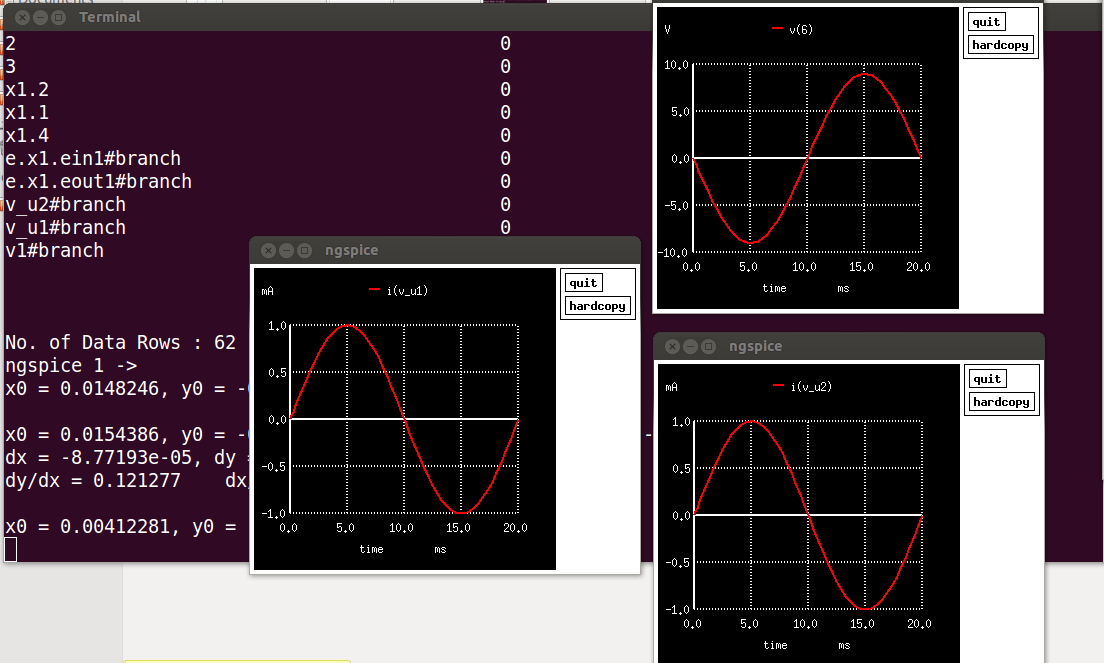
\includegraphics[width=1\linewidth]{figures/apd32.png}%If the fig is appearing too big/small, change the scaling factor 0.2
\caption{Ngspice Waveform}
\label{32}
\end{center}
\end{figure}

\item \textbf{Example 5.7:} For the circuit given in the figure \ref{33}, perform AC analysis where $R_1$ = 1k$\Omega$, $R_f$ = 100k$\Omega$, $C_f$ = 1.59nF and input voltage $V_i$ = 1V A.C.

\textbf{Solution:}
Create schematic and generate netlist in the same way as given in Example 2.1.
Click on ``analysis inserter" from Oscad tool bar.
select ``AC" and then enter the following details:
{\tt scale} = Lin, {\tt start frequency} = 1 , {\tt stop frequency} = 10 Meg, {\tt No. of points} = 10 as given in Figure \ref{34}. Click on ``Add Simulation Data" and save the analysis file.
For subcircuit builder, follow the steps given in Example 5.3.
Now click on {\tt Netlist Converter} and enter the value of AC source as shown in Figure \ref{35} and then press 'enter' key. Now click on Ngspice button in Toolbar. The figure \ref{36} will appear.

\begin{figure}%h stands for 'here'. If h is removed then the fig will go to the bottom or to the next page.
\begin{center}
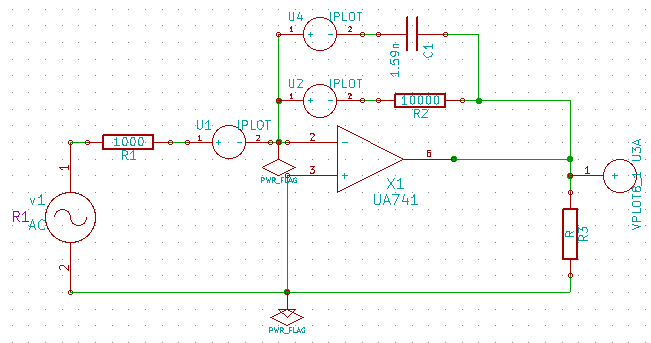
\includegraphics[width=1\linewidth]{figures/apd33.png}%If the fig is appearing too big/small, change the scaling factor 0.2
\caption{Schematic}
\label{33}
\end{center}
\end{figure}
\begin{figure}%h stands for 'here'. If h is removed then the fig will go to the bottom or to the next page.
\begin{center}
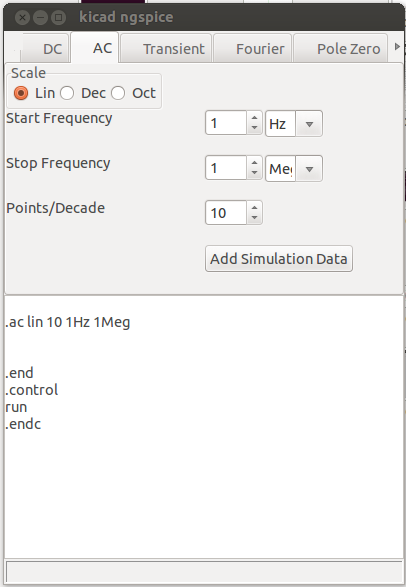
\includegraphics[width=1\linewidth]{figures/apd34.png}%If the fig is appearing too big/small, change the scaling factor 0.2
\caption{Analysis Inserter}
\label{34}
\end{center}
\end{figure}
\begin{figure}%h stands for 'here'. If h is removed then the fig will go to the bottom or to the next page.
\begin{center}
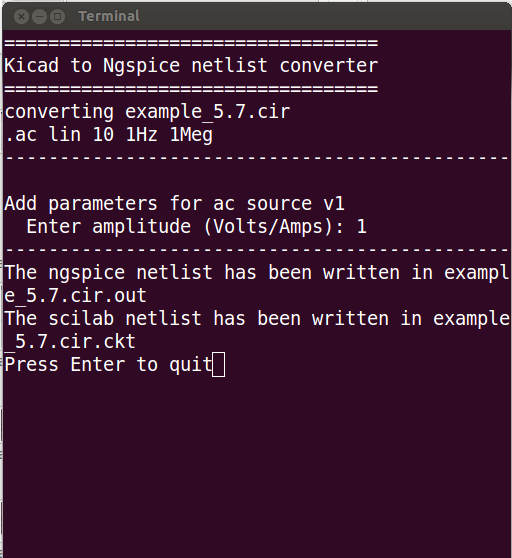
\includegraphics[width=1\linewidth]{figures/apd35.png}%If the fig is appearing too big/small, change the scaling factor 0.2
\caption{Kicad to Ngspice}
\label{35}
\end{center}
\end{figure}
\begin{figure}%h stands for 'here'. If h is removed then the fig will go to the bottom or to the next page.
\begin{center}
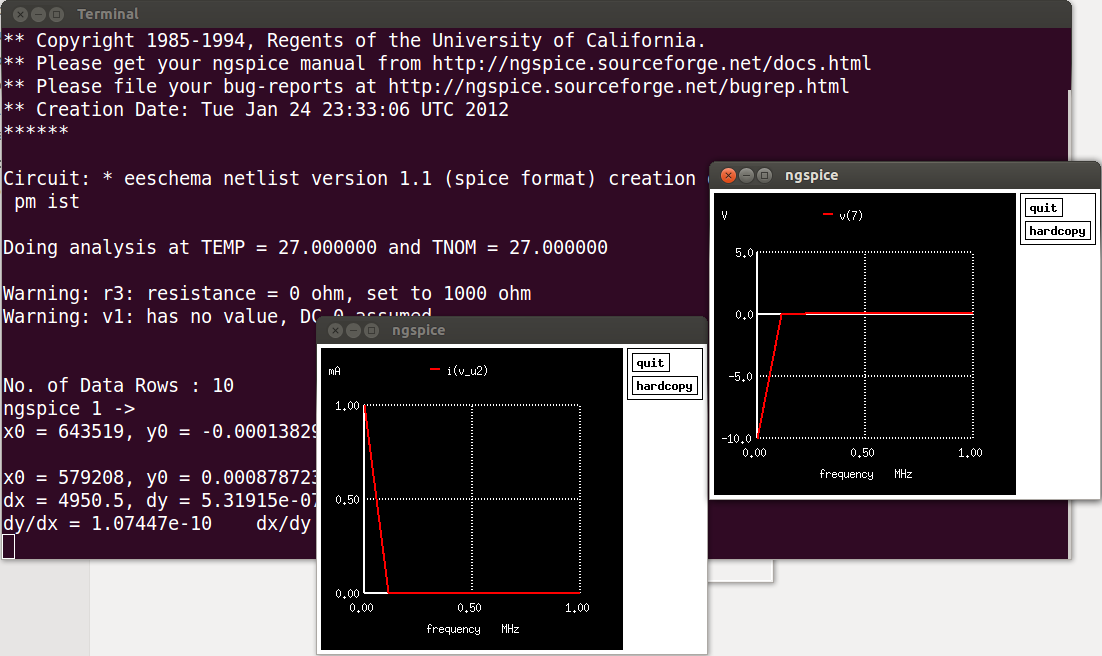
\includegraphics[width=1\linewidth]{figures/apd36.png}%If the fig is appearing too big/small, change the scaling factor 0.2
\caption{Ngspice Waveform}
\label{36}
\end{center}
\end{figure}
\end{enumerate}
\section {CMOS}

\textbf{Example 9.4:} Operation of CMOS Inverter\\


\textbf {Solution:} Create schematic and generate netlist in the same way as given in Example 2.1.
Click on ``analysis inserter" from Oscad tool bar.
select ``DC" and then enter the following details:
{\tt enter source name } = v1, {\tt start} = 0, {\tt increment} = 1 V, {\tt stop} = 15V as given in Figure \ref{38}. Click on ``Add Simulation Data" and save the analysis file. 

Now click on {\tt Netlist Converter} and enter the value of DC source as shown in Figure \ref{39} and then press 'enter' key. Now click on Ngspice button in Toolbar. The figure \ref{40} will appear.
\begin{figure}%h stands for 'here'. If h is removed then the fig will go to the bottom or to the next page.
\begin{center}
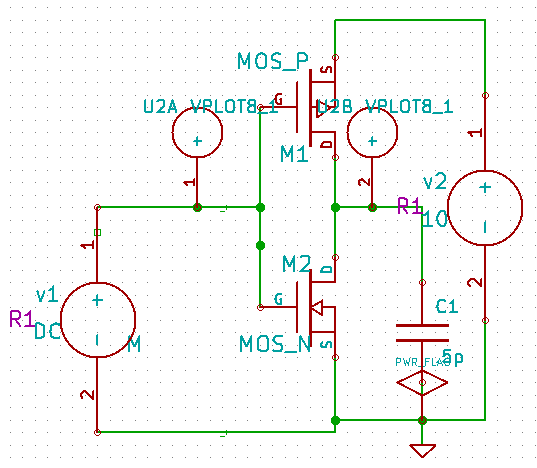
\includegraphics[width=1\linewidth]{figures/apd37.png}%If the fig is appearing too big/small, change the scaling factor 0.2
\caption{Schematic}
\label{37}
\end{center}
\end{figure}
\begin{figure}%h stands for 'here'. If h is removed then the fig will go to the bottom or to the next page.
\begin{center}
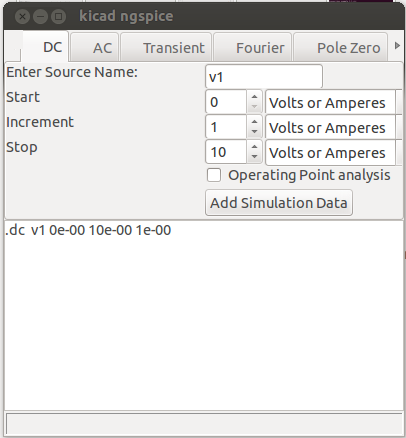
\includegraphics[width=1\linewidth]{figures/apd38.png}%If the fig is appearing too big/small, change the scaling factor 0.2
\caption{Analysis Inserter}
\label{38}
\end{center}
\end{figure}
\begin{figure}%h stands for 'here'. If h is removed then the fig will go to the bottom or to the next page.
\begin{center}
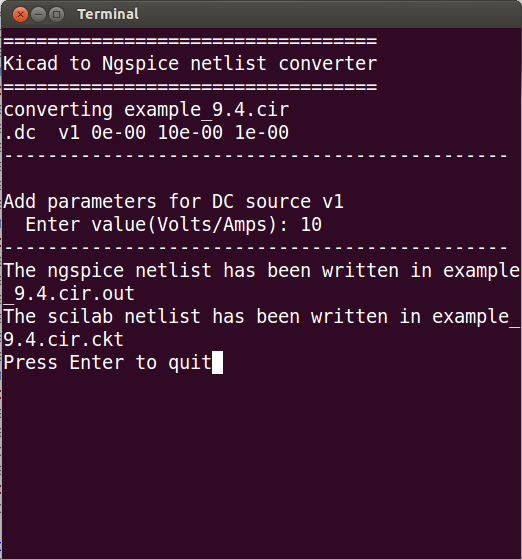
\includegraphics[width=1\linewidth]{figures/apd39.png}%If the fig is appearing too big/small, change the scaling factor 0.2
\caption{Kicad to Ngspice}
\label{39}
\end{center}
\end{figure}
\begin{figure}%h stands for 'here'. If h is removed then the fig will go to the bottom or to the next page.
\begin{center}
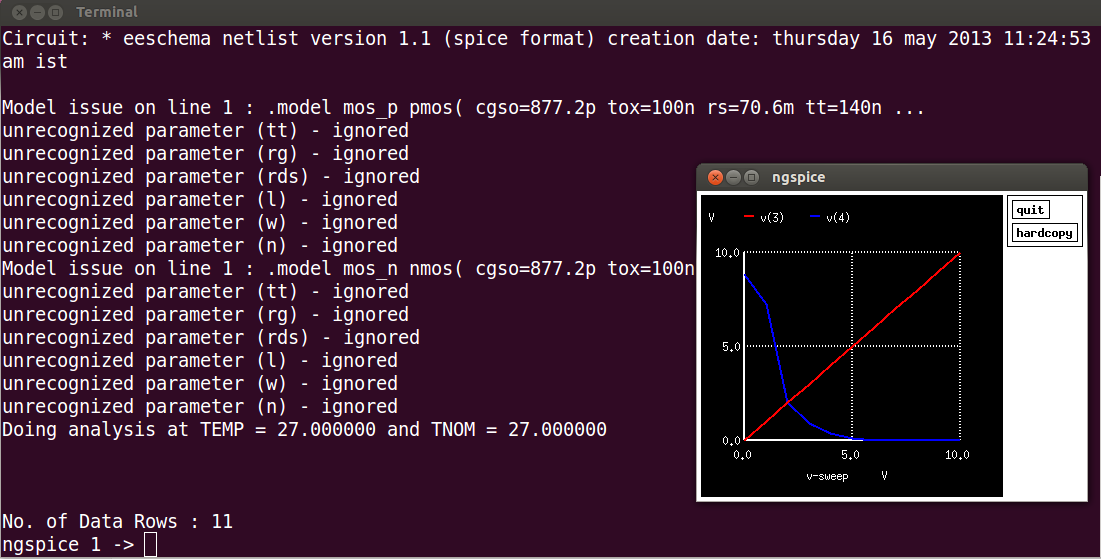
\includegraphics[width=1\linewidth]{figures/apd40.png}%If the fig is appearing too big/small, change the scaling factor 0.2
\caption{Ngspice Waveform}
\label{40}
\end{center}
\end{figure}







